\section{VALIDAÇÃO COM DATASETS PÚBLICOS}
\label{sec:validacao_datasets}

Como visto ao longo deste trabalho, o problema abordado envolve diversos tipos de restrições, tornando trabalhosa a troca de informações entre pesquisadores. Para solucionar esse problema, \citeonline{xhstt} sugeriu o XHSTT, um formato padronizado de arquivo XML para a representação de instâncias e soluções do \textit{High School Timetabling Problem}.

O projeto HSTT da \citeonline{Twente} hospeda publicamente diversas instâncias do problema no formato HXSTT. Destas, selecionaram-se três instâncias brasileiras para complementar a validação do sistema desenvolvido, utilizando dados externos. As próximas subções apresentarão cada instância e os resultados relacionados.

\subsection{Instância 1}

A primeira instância de teste, identificada como ``BrazilInstance1'', é composta por três turmas, 8 professores, cujas aulas devem ser alocadas em uma grade horária de 5 dias por semana, com 5 aulas por dia. As quantidade de aulas por professor em cada turma podem ser conferidas na tabela \ref{tab:config_aulas_br1}.

\begin{table}[h]
	\centering
	\caption[Configuração de Aulas - BrazilInstance1]{Configuração de Aulas - BrazilInstance1.
		\label{tab:config_aulas_br1}}
	\begin{tabular}{rrrrr}
		\toprule
		Professor & Matéria & S1 & S2 & S3 \\
		\midrule
		T1 & M1 & 3 & 3 & 3 \\
		T2 & M2 & 5 & 5 & 0 \\
		T3 & M3 & 3 & 3 & 3 \\
		T4 & M4 & 3 & 3 & 3 \\
		T5 & M5 & 0 & 5 & 5 \\
		T6 & M6 & 4 & 4 & 4 \\
		T7 & M7 & 5 & 0 & 5 \\
		T8 & M8 & 2 & 2 & 2 \\
		\bottomrule
	\end{tabular}
	\fonte{Autoria própria}
\end{table}


Os requisitos associados à instância são:
\begin{enumerate}
	\item Requisito 1 (obrigatório) : Não devem existir conflitos;
	\item Requisito 2 (obrigatório) : Não devem existir janelas;
	\item Requisito 3 (obrigatório) : Cada professor tem um dia da semana específico em que suas aulas não podem ser agendadas;
	\item Requisito 4 (não obrigatório) : Os professores T1, T2, T3, T4. T5, T7 e T8 não devem ser alocados em mais de 2 dias da semana;
	\item Requisito 5 (não obrigatório) : O professor T6 não deve ser alocado em mais de 3 dias da semana;
	\item Requisito 6 (não obrigatório) : Requisitos de quantidades mínimas de aulas duplas, que devido à sua extensão e não obrigatoriedade, não será explicitado.
\end{enumerate}

Sobre o requisito 3, a relação dos dias da semana bloqueados para cada professor pode ser conferida na lista abaixo:
\begin{enumerate}
	\item Segunda-feira: T5;
	\item Terça-feira: T4 e T7;
	\item Quarta-feira: T1 e T6;
	\item Quinta-feira: T3 e T8;
	\item Sexta-feira: T2.
\end{enumerate}

Dado um limite de execução de 10 segundos, o otimizador produziu como melhor solução a grade horária presente na figura \ref{fig:brazilinstance1_solucao}, cujas métricas de qualidade podem ser vistas no quadro \ref{qua:caracteristicas_horario_validacao_brazilinstance1}. Esta solução atende totalmente os requisitos obrigatórios da instância, e atende parcialmente os requisitos não obrigatórios.

\begin{figure}[h]
	\centering
	\caption{Grade exportada - Solução para a instância BrazilInstance1}
	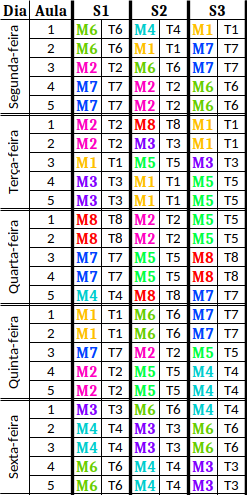
\includegraphics[width=0.5\textwidth]{./dados/figuras/brazilinstance1}
	\fonte{Autor}
	\label{fig:brazilinstance1_solucao}
\end{figure}

\begin{quadro}[h]
	\centering
	\caption{Métricas de qualidade da melhor solução - BrazilInstance1.\label{qua:caracteristicas_horario_validacao_brazilinstance1}}
	\begin{tabular}{|p{8cm}|p{1cm}|p{3cm}|}
		\hline
		\textbf{Nome} & \textbf{Valor} & \textbf{Tipo} \\
		Aulas desagrupadas & 0 & Rígida \\
		\hline
		Aulas em grupos de alinhamento não alinhadas & 0 & Rígida \\
		\hline
		Conflitos & 0 & Rígida \\
		\hline
		Dias com todos professores diferentes & 0 & Rígida \\
		\hline
		Erros nas regiões & 0 & Rígida \\
		\hline
		Excessos de aulas iguais & 0 & Rígida \\
		\hline
		Excessos de matérias iguais & 0 & Rígida \\
		\hline
		Horários com janela (total de todos professores) & 0 & Rígida \\
		\hline
		Limites diários violados & 0 & Rígida \\
		\hline
		Matérias desagrupadas & 0 & Rígida \\
		\hline
		Mínimos opcionais violados & 0 & Rígida \\
		\hline
		Mínimos violados & 0 & Rígida \\
		\hline
		Restrições violadas & 0 & Rígida \\
		\hline
		Excessos de dias trabalhados & 7 & Suave \\
		\hline
		Aulas separadas & 19 & Suave \\
		\hline
		Dias de professores sem aulas duplas & 2 & Suave \\
		\hline
		Matérias separadas & 19 & Suave \\
		\hline
		Número de grupos de alinhamento formados & 0 & Suave \\
		\hline
		Preferências não resolvidas & 0 & Suave \\
		\hline
		Restrições opcionais violadas & 0 & Suave \\
		\hline
	\end{tabular}
	\fonte{Autoria própria}
\end{quadro}

\clearpage
\subsection{Instância 2}

A segunda instância de teste, identificada como ``BrazilInstance5'', é composta por 13 turmas, 31 professores, cujas aulas devem ser alocadas em uma grade horária de 5 dias por semana, com 5 aulas por dia. As quantidade de aulas por professor em cada turma podem ser conferidas na tabela quadro \ref{tab:config_aulas_br5}.

\begin{table}[h]
	\centering
	\caption[Configuração de Aulas - BrazilInstance5]{Configuração de Aulas - BrazilInstance5.
		\label{tab:config_aulas_br5}}
	\begin{tabular}{rrrrrrrrrrrrrrr}
		\toprule
		Professor & Matéria & S1 & S2 & S3 & S4 & S5 & S6 & S7 & S8 & S9 & S 10 & S11 & S12 & S13 \\
		\midrule
		T1 & M1 & 6 & 6 & 6 & 0 & 0 & 0 & 0 & 0 & 0 & 0 & 0 & 0 & 0 \\
		T2 & M2 & 0 & 0 & 0 & 3 & 3 & 3 & 3 & 3 & 3 & 3 & 3 & 0 & 0 \\
		T3 & M3 & 0 & 0 & 0 & 0 & 0 & 0 & 0 & 0 & 0 & 0 & 0 & 3 & 0 \\
		T4 & M4 & 0 & 0 & 0 & 0 & 0 & 0 & 0 & 0 & 0 & 0 & 0 & 0 & 3 \\
		T5 & M5 & 0 & 0 & 0 & 0 & 0 & 0 & 0 & 0 & 0 & 0 & 0 & 2 & 0 \\
		T6 & M6 & 5 & 5 & 5 & 0 & 0 & 0 & 0 & 0 & 0 & 0 & 0 & 0 & 0 \\
		T7 & M7 & 0 & 0 & 0 & 4 & 4 & 4 & 4 & 4 & 0 & 0 & 0 & 0 & 0 \\
		T8 & M8 & 0 & 0 & 0 & 1 & 1 & 1 & 1 & 1 & 5 & 5 & 1 & 4 & 3 \\
		T9 & M9 & 0 & 0 & 0 & 0 & 0 & 0 & 0 & 0 & 0 & 0 & 4 & 0 & 0 \\
		T10 & M10 & 2 & 2 & 2 & 2 & 2 & 2 & 2 & 2 & 2 & 2 & 0 & 2 & 2 \\
		T11 & M11 & 0 & 0 & 0 & 0 & 0 & 0 & 0 & 0 & 0 & 0 & 2 & 0 & 0 \\
		T12 & M12 & 0 & 0 & 0 & 0 & 0 & 0 & 0 & 0 & 0 & 0 & 0 & 0 & 8 \\
		T13 & M13 & 2 & 2 & 2 & 0 & 0 & 0 & 0 & 0 & 0 & 0 & 0 & 0 & 0 \\
		T14 & M14 & 0 & 0 & 0 & 2 & 2 & 2 & 2 & 2 & 0 & 0 & 0 & 0 & 0 \\
		T15 & M15 & 0 & 0 & 0 & 0 & 0 & 0 & 0 & 0 & 2 & 2 & 2 & 2 & 0 \\
		T16 & M16 & 1 & 1 & 1 & 0 & 0 & 0 & 0 & 0 & 0 & 0 & 0 & 0 & 0 \\
		T17 & M17 & 3 & 3 & 3 & 0 & 0 & 0 & 0 & 0 & 0 & 0 & 0 & 0 & 0 \\
		T18 & M18 & 3 & 3 & 3 & 2 & 2 & 0 & 0 & 2 & 0 & 2 & 2 & 0 & 0 \\
		T19 & M19 & 3 & 3 & 3 & 0 & 0 & 2 & 2 & 0 & 2 & 0 & 0 & 2 & 0 \\
		T20 & M20 & 0 & 0 & 0 & 0 & 0 & 0 & 0 & 2 & 0 & 2 & 0 & 0 & 0 \\
		T21 & M21 & 0 & 0 & 0 & 0 & 0 & 0 & 0 & 0 & 2 & 0 & 2 & 2 & 0 \\
		T22 & M22 & 0 & 0 & 0 & 2 & 2 & 2 & 2 & 0 & 0 & 0 & 0 & 0 & 0 \\
		T23 & M23 & 0 & 0 & 0 & 3 & 3 & 3 & 3 & 0 & 0 & 0 & 3 & 0 & 0 \\
		T24 & M24 & 0 & 0 & 0 & 0 & 0 & 0 & 0 & 3 & 3 & 3 & 0 & 0 & 0 \\
		T25 & M25 & 0 & 0 & 0 & 3 & 3 & 3 & 3 & 3 & 3 & 0 & 0 & 0 & 0 \\
		T26 & M26 & 0 & 0 & 0 & 0 & 0 & 0 & 0 & 0 & 0 & 3 & 3 & 2 & 0 \\
		T27 & M27 & 0 & 0 & 0 & 3 & 0 & 0 & 0 & 0 & 0 & 3 & 3 & 0 & 0 \\
		T28 & M28 & 0 & 0 & 0 & 0 & 3 & 3 & 3 & 3 & 3 & 0 & 0 & 3 & 0 \\
		T29 & M29 & 0 & 0 & 0 & 0 & 0 & 0 & 0 & 0 & 0 & 0 & 0 & 0 & 8 \\
		T30 & M30 & 0 & 0 & 0 & 0 & 0 & 0 & 0 & 0 & 0 & 0 & 0 & 1 & 1 \\
		T31 & M31 & 0 & 0 & 0 & 0 & 0 & 0 & 0 & 0 & 0 & 0 & 0 & 2 & 0 \\
		\bottomrule
	\end{tabular}
	\fonte{Autoria própria}
\end{table}


\newpage
Os requisitos associados à instância são:
\begin{enumerate}
	\item Requisito 1 (obrigatório) : Não devem existir conflitos;
	\item Requisito 2 (não obrigatório) : Não devem existir janelas;
	\item Requisito 3 (não obrigatório) : Cada professor tem um l trabalhados por semana, conforme o quadro \ref{qua:limites_dias_trabalhados_brazilinstance5};
	\item Requisito 4 (não obrigatório) : Requisitos de quantidades mínimas de aulas duplas, o qual devido à sua extensão e não obrigatoriedade, não será explicitado.
\end{enumerate}

\begin{quadro}[h]
	\centering
	\caption{Limite de dias trabalhados por professor - BrazilInstance5.\label{qua:limites_dias_trabalhados_brazilinstance5}}
	\begin{tabular}{|p{2cm}|p{4cm}|}
		\hline
		\textbf{Professor} & \textbf{Limite em dias} \\
		\hline
		T1 & 4 \\
		\hline
		T2 & 5 \\
		\hline
		T3 & 2 \\
		\hline
		T4 & 2 \\
		\hline
		T5 & 1 \\
		\hline
		T6 & 3 \\
		\hline
		T7 & 4 \\
		\hline
		T8 & 5 \\
		\hline
		T9 & 2 \\
		\hline
		T10 & 5 \\
		\hline
		T11 & 2 \\
		\hline
		T12 & 4 \\
		\hline
		T13 & 2 \\
		\hline
		T14 & 2 \\
		\hline
		T15 & 2 \\
		\hline
		T16 & 1 \\
		\hline
		T17 & 2 \\
		\hline
		T18 & 4 \\
		\hline
		T19 & 4 \\
		\hline
		T20 & 1 \\
		\hline
		T21 & 2 \\
		\hline
		T22 & 2 \\
		\hline
		T23 & 3 \\
		\hline
		T24 & 2 \\
		\hline
		T25 & 4 \\
		\hline
		T26 & 2 \\
		\hline
		T27 & 2 \\
		\hline
		T28 & 4 \\
		\hline
		T29 & 4 \\
		\hline
		T30 & 1 \\
		\hline
		T31 & 1 \\
		\hline
	\end{tabular}
	\fonte{Autoria própria}
\end{quadro}

Dado um limite de execução de 60 segundos, o otimizador produziu como melhor solução a grade horária presente na figura \ref{fig:brazilinstance5_solucao}, cujas métricas de qualidade podem ser vistas no quadro \ref{qua:caracteristicas_horario_validacao_brazilinstance5}. Esta solução atende totalmente os requisitos 1 e 3, e atende parcialmente os requisitos não obrigatórios 2 e 4.

\begin{figure}[h]
	\centering
	\caption{Grade exportada - Solução para a instância BrazilInstance5}
	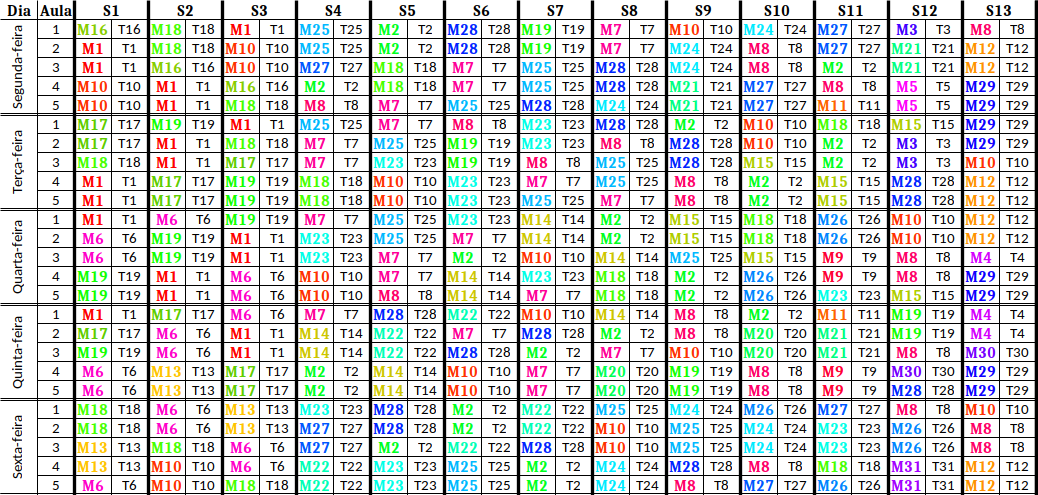
\includegraphics[width=1\textwidth]{./dados/figuras/brazilinstance5}
	\fonte{Autor}
	\label{fig:brazilinstance5_solucao}
\end{figure}

\begin{quadro}[h]
	\centering
	\caption{Métricas de qualidade da melhor solução - BrazilInstance5.\label{qua:caracteristicas_horario_validacao_brazilinstance5}}
	\begin{tabular}{|p{8cm}|p{1cm}|p{3cm}|}
		\hline
		\textbf{Nome} & \textbf{Valor} & \textbf{Tipo} \\
		Aulas desagrupadas & 0 & Rígida \\
		\hline
		Aulas em grupos de alinhamento não alinhadas & 0 & Rígida \\
		\hline
		Conflitos & 0 & Rígida \\
		\hline
		Dias com todos professores diferentes & 0 & Rígida \\
		\hline
		Erros nas regiões & 0 & Rígida \\
		\hline
		Excessos de aulas iguais & 0 & Rígida \\
		\hline
		Excessos de matérias iguais & 0 & Rígida \\
		\hline
		Limites diários violados & 0 & Rígida \\
		\hline
		Matérias desagrupadas & 0 & Rígida \\
		\hline
		Mínimos opcionais violados & 0 & Rígida \\
		\hline
		Mínimos violados & 0 & Rígida \\
		\hline
		Restrições violadas & 0 & Rígida \\
		\hline
		Excessos de dias trabalhados & 0 & Suave \\
		\hline
		Horários com janela (total de todos professores) & 11 & Suave \\
		\hline
		Aulas separadas & 99 & Suave \\
		\hline
		Dias de professores sem aulas duplas & 24 & Suave \\
		\hline
		Matérias separadas & 99 & Suave \\
		\hline
		Número de grupos de alinhamento formados & 0 & Suave \\
		\hline
		Preferências não resolvidas & 0 & Suave \\
		\hline
		Restrições opcionais violadas & 0 & Suave \\
		\hline
	\end{tabular}
	\fonte{Autoria própria}
\end{quadro}

\clearpage
\subsection{Instância 3}

A terceira instância de teste, identificada como ``BrazilInstance7'', é composta por 20 turmas, 33 professores, cujas aulas devem ser alocadas em uma grade horária de 5 dias por semana, com 5 aulas por dia. As quantidade de aulas por professor em cada turma podem ser conferidas nas tabelas \ref{tab:config_aulas_br7} e \ref{tab:config_aulas_br7_2}.

\begin{table}[h]
	\centering
	\caption[Configuração de Aulas das turmas S1 a S10 - BrazilInstance7]{Configuração de Aulas - BrazilInstance7.
		\label{tab:config_aulas_br7}}
	\begin{tabular}{rrrrrrrrrrrr}
		\toprule
		Professor & Matéria & S1 & S2 & S3 & S4 & S5 & S6 & S7 & S8 & S9 & S10 \\
		\midrule
		T1 & M1 & 3 & 3 & 3 & 3 & 0 & 0 & 0 & 0 & 0 & 0 \\
		T2 & M2 & 0 & 0 & 0 & 0 & 0 & 0 & 3 & 3 & 3 & 4 \\
		T3 & M3 & 0 & 0 & 0 & 0 & 0 & 0 & 0 & 0 & 0 & 0 \\
		T4 & M4 & 0 & 0 & 0 & 0 & 3 & 3 & 0 & 0 & 0 & 0 \\
		T5 & M5 & 4 & 4 & 4 & 4 & 0 & 0 & 0 & 0 & 0 & 0 \\
		T6 & M6 & 0 & 0 & 0 & 0 & 4 & 4 & 4 & 4 & 0 & 1 \\
		T7 & M7 & 0 & 0 & 0 & 0 & 0 & 0 & 0 & 0 & 4 & 4 \\
		T8 & M8 & 0 & 0 & 0 & 0 & 0 & 0 & 0 & 0 & 0 & 0 \\
		T9 & M9 & 0 & 0 & 0 & 0 & 0 & 0 & 0 & 0 & 0 & 0 \\
		T10 & M10 & 3 & 3 & 3 & 3 & 3 & 0 & 0 & 0 & 0 & 0 \\
		T11 & M11 & 0 & 0 & 0 & 0 & 0 & 3 & 3 & 3 & 3 & 3 \\
		T12 & M12 & 0 & 0 & 0 & 0 & 0 & 0 & 0 & 0 & 0 & 0 \\
		T13 & M13 & 0 & 0 & 0 & 0 & 0 & 0 & 0 & 0 & 0 & 0 \\
		T14 & M14 & 3 & 3 & 3 & 0 & 0 & 0 & 0 & 0 & 0 & 3 \\
		T15 & M15 & 0 & 0 & 0 & 3 & 3 & 3 & 0 & 0 & 0 & 0 \\
		T16 & M16 & 0 & 0 & 0 & 0 & 0 & 0 & 3 & 3 & 3 & 0 \\
		T17 & M17 & 3 & 3 & 3 & 0 & 0 & 0 & 0 & 0 & 0 & 2 \\
		T18 & M18 & 0 & 0 & 0 & 3 & 3 & 3 & 0 & 0 & 0 & 0 \\
		T19 & M19 & 0 & 0 & 0 & 0 & 0 & 0 & 3 & 3 & 3 & 0 \\
		T20 & M20 & 2 & 2 & 2 & 2 & 2 & 2 & 2 & 0 & 0 & 0 \\
		T21 & M21 & 0 & 0 & 0 & 0 & 0 & 0 & 0 & 2 & 2 & 2 \\
		T22 & M22 & 0 & 0 & 0 & 0 & 0 & 0 & 0 & 0 & 0 & 0 \\
		T23 & M23 & 2 & 2 & 2 & 0 & 0 & 0 & 0 & 0 & 0 & 2 \\
		T24 & M24 & 0 & 0 & 0 & 2 & 2 & 2 & 0 & 0 & 0 & 0 \\
		T25 & M25 & 0 & 0 & 0 & 0 & 0 & 0 & 2 & 2 & 2 & 0 \\
		T26 & M26 & 2 & 0 & 0 & 2 & 0 & 0 & 2 & 0 & 0 & 2 \\
		T27 & M27 & 0 & 2 & 0 & 0 & 2 & 0 & 0 & 2 & 0 & 0 \\
		T28 & M28 & 0 & 0 & 2 & 0 & 0 & 2 & 0 & 0 & 2 & 0 \\
		T29 & M29 & 2 & 0 & 0 & 2 & 0 & 0 & 2 & 0 & 0 & 2 \\
		T30 & M30 & 0 & 2 & 0 & 0 & 2 & 0 & 0 & 2 & 0 & 0 \\
		T31 & M31 & 0 & 0 & 2 & 0 & 0 & 2 & 0 & 0 & 2 & 0 \\
		T32 & M32 & 1 & 1 & 1 & 1 & 1 & 1 & 1 & 1 & 1 & 0 \\
		T33 & M33 & 0 & 0 & 0 & 0 & 0 & 0 & 0 & 0 & 0 & 0 \\
		\bottomrule
	\end{tabular}
	\fonte{Dataset hospedado pela Universidade de \citeonline{Twente}}
\end{table}

\begin{table}[h]
	\centering
	\caption[Configuração de Aulas das turmas S11 a S20 - BrazilInstance7]{Configuração de Aulas - BrazilInstance7.
		\label{tab:config_aulas_br7_2}}
	\begin{tabular}{rrrrrrrrrrrr}
		\toprule
		Professor & Matéria & S11 & S12 & S13 & S14 & S15 & S16 & S17 & S18 & S19 & S20 \\
		\midrule
		T1 & M1 & 0 & 0 & 0 & 0 & 0 & 4 & 4 & 0 & 0 & 0 \\
		T2 & M2 & 4 & 0 & 0 & 0 & 0 & 0 & 0 & 0 & 0 & 0 \\
		T3 & M3 & 0 & 4 & 4 & 4 & 4 & 0 & 0 & 0 & 0 & 0 \\
		T4 & M4 & 0 & 0 & 0 & 0 & 0 & 0 & 0 & 4 & 4 & 4 \\
		T5 & M5 & 0 & 0 & 0 & 1 & 0 & 0 & 0 & 0 & 0 & 0 \\
		T6 & M6 & 0 & 1 & 0 & 0 & 0 & 0 & 0 & 0 & 0 & 0 \\
		T7 & M7 & 4 & 4 & 1 & 0 & 0 & 0 & 0 & 0 & 0 & 0 \\
		T8 & M8 & 1 & 0 & 4 & 4 & 4 & 4 & 0 & 0 & 0 & 0 \\
		T9 & M9 & 0 & 0 & 0 & 0 & 1 & 0 & 4 & 4 & 4 & 4 \\
		T10 & M10 & 0 & 0 & 0 & 0 & 0 & 0 & 0 & 0 & 0 & 0 \\
		T11 & M11 & 0 & 0 & 0 & 0 & 0 & 0 & 0 & 0 & 0 & 0 \\
		T12 & M12 & 3 & 3 & 3 & 3 & 3 & 0 & 0 & 0 & 0 & 0 \\
		T13 & M13 & 0 & 0 & 0 & 0 & 0 & 3 & 3 & 3 & 3 & 3 \\
		T14 & M14 & 0 & 0 & 3 & 0 & 0 & 2 & 2 & 0 & 0 & 0 \\
		T15 & M15 & 3 & 0 & 0 & 3 & 0 & 0 & 0 & 2 & 2 & 0 \\
		T16 & M16 & 0 & 3 & 0 & 0 & 3 & 0 & 0 & 0 & 0 & 2 \\
		T17 & M17 & 0 & 0 & 2 & 0 & 0 & 2 & 2 & 0 & 0 & 0 \\
		T18 & M18 & 2 & 0 & 0 & 2 & 0 & 0 & 0 & 2 & 2 & 0 \\
		T19 & M19 & 0 & 2 & 0 & 0 & 2 & 0 & 0 & 0 & 0 & 2 \\
		T20 & M20 & 0 & 0 & 0 & 0 & 0 & 0 & 0 & 0 & 0 & 0 \\
		T21 & M21 & 2 & 2 & 2 & 2 & 0 & 0 & 0 & 0 & 0 & 0 \\
		T22 & M22 & 0 & 0 & 0 & 0 & 2 & 2 & 2 & 2 & 2 & 2 \\
		T23 & M23 & 2 & 2 & 0 & 0 & 0 & 0 & 0 & 0 & 2 & 0 \\
		T24 & M24 & 0 & 0 & 2 & 2 & 2 & 0 & 0 & 0 & 0 & 2 \\
		T25 & M25 & 0 & 0 & 0 & 0 & 0 & 2 & 2 & 2 & 0 & 0 \\
		T26 & M26 & 0 & 0 & 2 & 0 & 0 & 2 & 0 & 0 & 2 & 0 \\
		T27 & M27 & 2 & 0 & 0 & 2 & 0 & 0 & 2 & 0 & 0 & 2 \\
		T28 & M28 & 0 & 2 & 0 & 0 & 2 & 0 & 0 & 2 & 0 & 0 \\
		T29 & M29 & 0 & 0 & 2 & 0 & 0 & 2 & 0 & 0 & 2 & 0 \\
		T30 & M30 & 2 & 0 & 0 & 2 & 0 & 0 & 2 & 0 & 0 & 0 \\
		T31 & M31 & 0 & 2 & 0 & 0 & 2 & 0 & 0 & 2 & 0 & 2 \\
		T32 & M32 & 0 & 0 & 0 & 0 & 0 & 1 & 1 & 1 & 1 & 1 \\
		T33 & M33 & 0 & 0 & 0 & 0 & 0 & 1 & 1 & 1 & 1 & 1 \\
		\bottomrule
	\end{tabular}
	\fonte{Dataset hospedado pela Universidade de \citeonline{Twente}}
\end{table}



\newpage
Os requisitos associados à instância são:
\begin{enumerate}
	\item Requisito 1 (obrigatório) : Não devem existir conflitos;
	\item Requisito 2 (não obrigatório) : Não devem existir janelas;
	\item Requisito 3 (não obrigatório) : Cada professor tem um limite de dias trabalhados por semana, conforme o quadro \ref{qua:limites_dias_trabalhados_brazilinstance7};
	\item Requisito 4 (não obrigatório) : Requisitos de quantidades mínimas de aulas duplas, o qual devido à sua extensão e não obrigatoriedade, não será explicitado.
\end{enumerate}

\begin{quadro}[h]
	\centering
	\caption{Limite de dias trabalhados por professor - BrazilInstance7.\label{qua:limites_dias_trabalhados_brazilinstance7}}
	\begin{tabular}{|p{2cm}|p{4cm}|}
		\hline
		\textbf{Professor} & \textbf{Limite em dias} \\
		\hline
		T1 & 4 \\
		\hline
		T2 & 4 \\
		\hline
		T3 & 4 \\
		\hline
		T4 & 4 \\
		\hline
		T5 & 4 \\
		\hline
		T6 & 4 \\
		\hline
		T7 & 4 \\
		\hline
		T8 & 4 \\
		\hline
		T9 & 4 \\
		\hline
		T10 & 3 \\
		\hline
		T11 & 3 \\
		\hline
		T12 & 3 \\
		\hline
		T13 & 3 \\
		\hline
		T14 & 4 \\
		\hline
		T15 & 4 \\
		\hline
		T16 & 4 \\
		\hline
		T17 & 4 \\
		\hline
		T18 & 4 \\
		\hline
		T19 & 3 \\
		\hline
		T20 & 3 \\
		\hline
		T21 & 3 \\
		\hline
		T22 & 3 \\
		\hline
		T23 & 3 \\
		\hline
		T24 & 3 \\
		\hline
		T25 & 3 \\
		\hline
		T26 & 3 \\
		\hline
		T27 & 3 \\
		\hline
		T28 & 3 \\
		\hline
		T29 & 3 \\
		\hline
		T30 & 3 \\
		\hline
		T31 & 3 \\
		\hline
		T32 & 3 \\
		\hline
		T33 & 1 \\
		\hline
	\end{tabular}
	\fonte{Autoria própria}
\end{quadro}

\newpage
A melhor solução gerada em um intervalo de 60 segundos pode ser vista nas figuras \ref{fig:brazilinstance7_solucao} e \ref{fig:brazilinstance7_solucao_2}. Vale ressaltar que todas as salas da instância pertecem ao mesmo turno, ou seja, apesar de as turmas terem sido separadas em duas figuras para melhor legibilidade, ainda poderiam ocorrer conflitos entre as turmas S1 e S20, por exemplo.

As métricas de qualidade desta solução podem ser observadas no quadro \ref{qua:caracteristicas_horario_validacao_brazilinstance7}, e indicam que foram atendidos totalmente os requisitos 1 e 3, e parcialmente atendidos os requisitos não obrigatórios 2 e 4.

\begin{figure}[h]
	\centering
	\caption{Solução para a instância BrazilInstance7 - Turmas S1 a S10}
	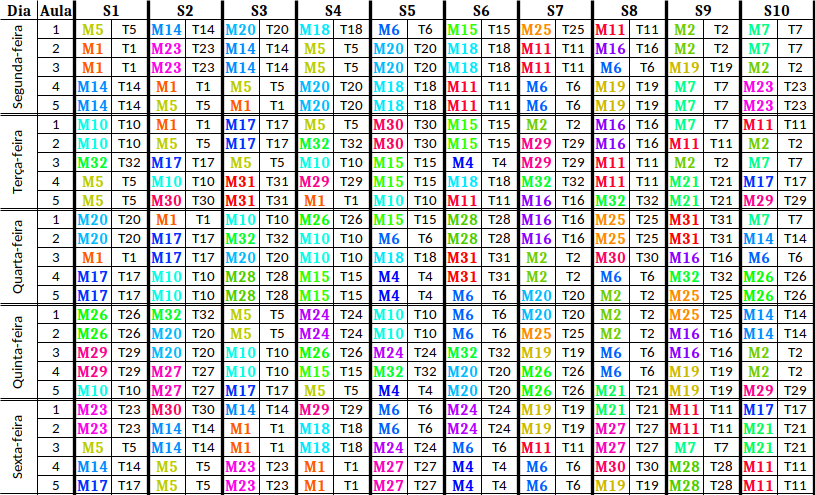
\includegraphics[width=1\textwidth]{./dados/figuras/brazilinstance7}
	\fonte{Autor}
	\label{fig:brazilinstance7_solucao}
\end{figure}

\begin{figure}[h]
	\centering
	\caption{Solução para a instância BrazilInstance7 - Turmas S11 a S20}
	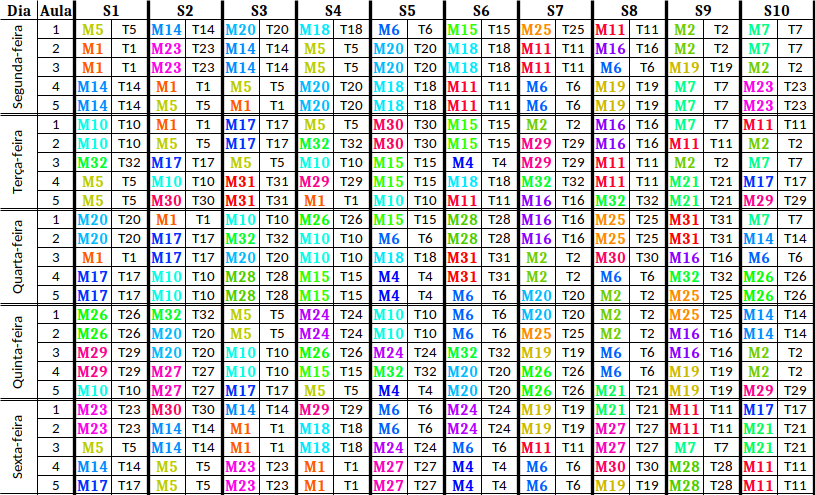
\includegraphics[width=1\textwidth]{./dados/figuras/brazilinstance7}
	\fonte{Autor}
	\label{fig:brazilinstance7_solucao_2}
\end{figure}

\begin{quadro}[h]
	\centering
	\caption{Métricas de qualidade da melhor solução - BrazilInstance7.\label{qua:caracteristicas_horario_validacao_brazilinstance7}}
	\begin{tabular}{|p{8cm}|p{1cm}|p{3cm}|}
		\hline
		\textbf{Nome} & \textbf{Valor} & \textbf{Tipo} \\
		\hline
		Aulas desagrupadas & 0 & Rígida \\
		\hline
		Aulas em grupos de alinhamento não alinhadas & 0 & Rígida \\
		\hline
		Conflitos & 0 & Rígida \\
		\hline
		Dias com todos professores diferentes & 0 & Rígida \\
		\hline
		Erros nas regiões & 0 & Rígida \\
		\hline
		Excessos de aulas iguais & 0 & Rígida \\
		\hline
		Excessos de matérias iguais & 0 & Rígida \\
		\hline
		Limites diários violados & 0 & Rígida \\
		\hline
		Matérias desagrupadas & 0 & Rígida \\
		\hline
		Mínimos opcionais violados & 0 & Rígida \\
		\hline
		Mínimos violados & 0 & Rígida \\
		\hline
		Restrições violadas & 0 & Rígida \\
		\hline
		Excessos de dias trabalhados & 3 & Suave \\
		\hline
		Aulas separadas & 164 & Suave \\
		\hline
		Dias de professores sem aulas duplas & 43 & Suave \\
		\hline
		Horários com janela (total de todos professores) & 20 & Suave \\
		\hline
		Matérias separadas & 164 & Suave \\
		\hline
		Número de grupos de alinhamento formados & 0 & Suave \\
		\hline
		Preferências não resolvidas & 0 & Suave \\
		\hline
		Restrições opcionais violadas & 0 & Suave \\
		\hline
	\end{tabular}
	\fonte{Autoria própria}
\end{quadro}